\documentclass{standalone}

\usepackage{amssymb}
\usepackage{amsthm}
\usepackage{amsmath}


\usepackage{tikz}
\usetikzlibrary{shapes,backgrounds,calc,patterns}
\usepackage{venndiagram}


\begin{document}
	\usetikzlibrary{arrows}
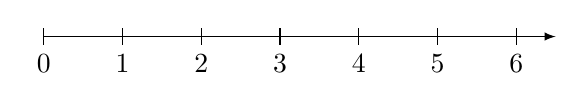
\begin{tikzpicture}[scale=1]
\draw[-latex] (0,0) -- (6.5,0) ;
\foreach \x in  {0,1,2,3,4,5,6}
\draw[shift={(\x,0)},color=black] (0pt,3pt) -- (0pt,-3pt);
\foreach \x in {0,1,2,3,4,5,6}
\draw[shift={(\x,0)},color=black] (0pt,0pt) -- (0pt,-3pt) node[below] {\(\x\)};
\end{tikzpicture}

\end{document}